\documentclass[border=6pt]{standalone}
\usepackage{amsmath}
\usepackage{amssymb}
\usepackage{tikz}
\usepackage{pgfplots}
\pgfplotsset{compat=1.18}
\usetikzlibrary{arrows.meta,calc,positioning}
\begin{document}
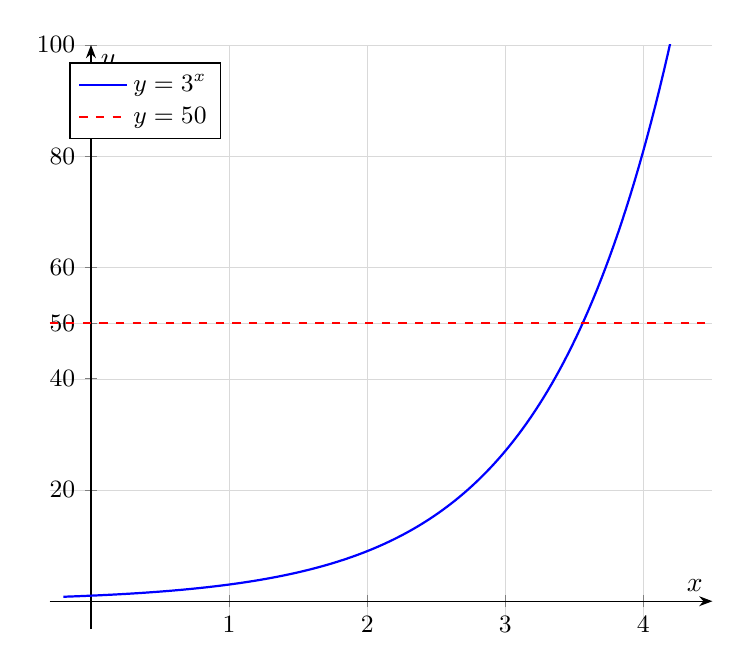
\begin{tikzpicture}
\begin{axis}[
    axis lines = middle,
    xlabel = {$x$}, ylabel = {$y$},
    grid=both,
    grid style={line width=.1pt, draw=gray!30},
    axis line style={-Stealth},
    legend style={font=\small},
    tick label style={font=\small},
    xmin=-0.3, xmax=4.5, ymin=-5, ymax=100,
    xtick={0,1,2,3,4},
    ytick={0,20,40,50,60,80,100},
    width=10cm, height=9cm,
    legend pos=north west,
]
\addplot[domain=-0.2:4.3, samples=150, thick, blue] {3^x};
\addlegendentry{$y=3^x$}
\addplot[domain=-0.3:4.5, samples=2, thick, red, dashed] {50};
\addlegendentry{$y=50$}
\end{axis}
\end{tikzpicture}
\end{document}
